\color{finishing}

\section{Konzeption}

In diesem Kapitel werden die Anforderungsdefinitionen des Projektes, mit Spezialisierung auf die verschiedenen Use Cases beschrieben.

\subsection{Anforderunsdefinitionen}

Ein Schwarmverhalten zur Interaktion von Kleinroboter benötigt verschiedene Anforderungen, um korrekt untereinander agieren zu können. Die Basis hierbei bildet das Kommunikationssystem zwischen den einzelnen Komponenten, um erfasste Daten zuverlässig zu synchronisieren. Um die Daten entsprechend zu interpretieren benötigt jede Komponente den jeweiligen Aufbau der Kommunikation, damit diese verwertet und Aktionen ausgeführt werden können.\\
Diese Aktionen repräsentieren den Grundbestandteil des Schwarmverhaltens und sind auf die verschiedenen Systeme verteilt. Die Roboter benötigen hierbei implementierte Funktionen, wie das Ansteuern von Motoren, Sensorik, sowie die Aktualisierung, um erfasste Daten an Nutzer weiterzuleiten. Zur Steuerung dient eine App für mobile Smartphones mit einem \gls{ui} um verschiedene Szenarien zu starten, sowie die Roboter kontrollieren zu können. Die Kontrollschnittstelle stellt dabei eine Desktopanwendung dar, über die der Nutzer mit den Robotern kommuniziert und Daten zur Steuerung abgreifen kann, wobei mehrere Nutzer zur selben Zeit mit verschiedenen Szenarien unterstützt werden sollen.\\

\noindent
Damit bestehen folgende Anforderungsdefinitionen an die zu erstellenden Softwarekomponenten:
\begin{itemize}
	\item Kommunikationssystem
	\item Interpretation
	\item \gls{ui}
	\item Steuerungsfunktionen
\end{itemize}

\newpage
\subsection{Softwarearchitektur}

Die Architektur des Schwarmverhaltens besteht aus drei Hauptkomponente, den Robotern, einer Desktopanwendung, sowie einer mobilen App, siehe Abbildung \ref{fig:softwarearchitecture}.\\
Diese Komponenten kommunizieren über ein drahtloses Netzwerk mittels \gls{tcp} untereinander, indem diese Zeichenketten als \gls{json} versenden. Dadurch lassen sich gesammelte Daten als Objekte kapseln und auf den verschiedenen Systemen entsprechend synchronisieren. Dies geschieht über eine Klassenstruktur, die Kommandos abbildet, durch die die kommunizierten Daten serialisiert und als Objekte dargestellt werden können, siehe \ref{kommunikation}.\\
Die Roboter basieren auf dem Java System \gls{lejos}, da durch die bereitgestellten Bibliotheken für \gls{ev3} Systeme eine unkomplizierte Implementierung von Logik möglich ist, sowie eine direkte Unterstützung von \gls{eclipse} gegeben ist, um erstellte Software zu debuggen. Die Roboter unterstützen für ein Schwarmverhalten klassische Funktionen, um die Daten der vorhandenen Sensorik auszulesen, sowie Motoren anzusteuern. Diese Funktionen werden einerseits durch Kommandos ausgeführt um den entsprechenden Roboter zu steuern. Anderseits werden regelmäßig Daten durch einen Prozess erfasst, um diese auf dem Backend zu aktualisieren.\\
Die App beruht auf der plattformübergreifenden Implementierung mittels des Frameworks Xamarin um möglichst viele Systeme zu erreichen. Sie baut dabei auf ein einfaches \gls{ui} mit dem Design Pattern \gls{mvvm} auf, um diese von der eigentlichen Logik zu trennen und einen qualitativ hochwertigen Quellcode zu schaffen, der einfach gewartet werden kann. Die App besitzt Basisfunktionen zur Erstellung von Kommandos, die die Verwaltung von Szenarien veranlassen und steuert somit den Schwarm.\\
Das Backend dient als Kommunikationsschnittstelle des gesamten Systems und steuert die Kommandos für den Ablauf der Szenarien. Es besitzt ein \gls{ui} mit \gls{javafx} Realisierung zur Anzeige von erfassten Daten der einzelnen Komponenten und stellt diese anhand einer auswählbaren Hierarchie dar.

\newpage
\begin{verbatim}
\end{verbatim}
\begin{figure}[h]
	\centering
	\includegraphics[width=0.65\textwidth]{images/konzeption/Softwarearchitecture.png}
	\caption{Softwarearchitektur}
	\label{fig:softwarearchitecture}
\end{figure}

\newpage
\subsection{Steuerung}

Die Steuerung des Roboterschwarms greift in sämtlich implementierten Szenarien auf die Sensorik des Smartphones als Basis zurück. Verwendet werden hierbei die Bewegungssensoren um eine Steuerung durch das Hin- und Herschwenken des Smartphones zu ermöglichen. Dies stellt eine intuitive Steuerung dar und ist für jeden neuen Nutzer schnell begreiflich. In Abbildung \ref{fig:steuerung} ist die entsprechende Steuerung zur Bewegung des Roboters dargestellt. Um die Roboter möglichst genau zu steuern, erfasst die Sensorik laufend Daten, welche im \gls{ui} angezeigt werden. Dadurch lässt sich eine Veränderung der Daten darstellen, die zu einer signifikant verbesserten Steuerung führen.\\

\begin{figure}[h]
	\centering
	\includegraphics[width=0.7\textwidth]{images/Controling.png}
	\caption{Steuerung}
	\label{fig:steuerung}
\end{figure}

\subsection{Szenarien}

Zum Ablauf der Software greift der Roboterschwarm auf verschieden definierte Szenarien als Kontext zurück. Diese sind in Control, Synchron, Follow, Flee und Catch untergliedert, wobei ein Single mit einem Nutzer oder einem Mehrnutzersystem als Multi unterschieden wird. Der Multi Mode dient hierbei als Erweiterung zur Software und ist im vorliegenden System nicht implementiert und kann daher nicht genutzt werden. Folgend werden die einzelnen Szenarien beschrieben, die als Kontext für ein Schwarmverhalten genutzt werden können.

\paragraph{Control}

stellt eine direkte Steuerung eines einzelnen Roboters und fällt somit nicht unter die Kategorie Schwarmverherhalten. Dieses Szenario dient zur Entwicklung der grundlegenden Funktionen, auf denen das Schwarmverhalten und damit weitere Szenarien aufbauen.

\paragraph{Synchron}

stellt eine synchrone Steuerung von mehreren Robotern dar, in dessen Kontext jeder beteiligte Roboter identische Kommandos erhält. Durch eine entsprechende Aufstellung der Roboter lassen sich Schwärme aus dem Tierreich, wie Fische oder Vögel nachahmen.

\paragraph{Follow}

stellt eine Reihe von Robotern dar, indem der vorderste vom Nutzer gesteuert werden kann. Die restlichen Roboter erhalten ihrer Position in der Schlange entsprechend der Position ihres Vordermannes, zu dem diese vollkommen autonom fahren. Da diese Ablauf laufend wiederholt wird, stellen alle Roboter gesamt eine Schlange dar, wobei die einzelnen die Muskeln und der vorderste Roboter den Kopf repräsentiert.

\paragraph{Flee}

stellt ein Verfolgungsszenario dar, indem der Nutzer mit seinem Roboter vor anderen flieht. Dabei erhalten die restlichen Roboter laufend eine Position um immer näher an diesen heranzufahren. Sollte der Nutzer durch einen Roboter erwischt werden, ertönt ein Endsignal , wobei anschließend das Szenario beendet wird.

\paragraph{Catch}

stellt ein Verfolgungsszenario dar, indem der Nutzer die restlichen Roboter fängt. Diese fahren zufällig in verschiedene Richtungen davon. Sollte der Nutzer alle gefangen haben, ertönt ein Signal und beendet damit das Szenario.

\begin{figure}[h]
	\begin{center}
		
\includegraphics[width=0.4\textwidth]{images/logos/UWP/FleeAndCatch_Logo.png}
	\end{center}
	\caption{Logo}
	\label{fig:Logo}
\end{figure}

\newpage
\subsection{Use Cases}

In diesem Abschnitt werden die Use Cases des Schwarmverhaltens beschrieben. Dabei wird insbesondere auf den Ablauf in Form von \gls{uml} Diagrammen eingegangen.

\subsubsection{Connection}

Der Use Case Connection stellt den Ablauf eines Verbindungsaufbaus zwischen den Komponenten und der Desktopanwendung dar. Dies soll über die Nutzung eines drahtlosen Netzwerks mittels \gls{tcp} Schnittstelle des Smartphones realisiert werden. Die IP-Adresse kann dabei durch die Verwendung einer \gls{sqlite} Datenbank lokal gespeichert werden, um diese später bei einem erneuten Aufruf automatisch eintragen zu lassen. Zur Unterscheidung der verschiedenen Komponenten soll eine individuelle Identifikation erstellt werden, wobei der Typ der Komponente, sowie weitere Merkmale ersichtlich werden sollen.\\
Der Use Case soll dabei in zwei unterschiedliche Typen untergliedert werden, womit ein Verbindungsaufbau von einem Verbindungsabbau unterschieden werden kann. Der Ablauf eines Verbindungsaufbaus soll dabei für jede Komponente identisch 
abgewickelt werden, siehe Abbildung \ref{fig:UC_Connect}. Um eine entsprechend stabile Reaktionszeit der teilnehmenden Roboter zu garantieren, sollen zum Start des Verbindungsaufbaus wiederholt Kommandos versendet werden. Dies soll eine erhöhte \gls{cpu} Laufzeit erreichen, um eine Zeitverzögerung zur Laufzeit der Szenarios zu verhindern.\\

\begin{figure}[h]
	\centering
	\subfloat[Log in]{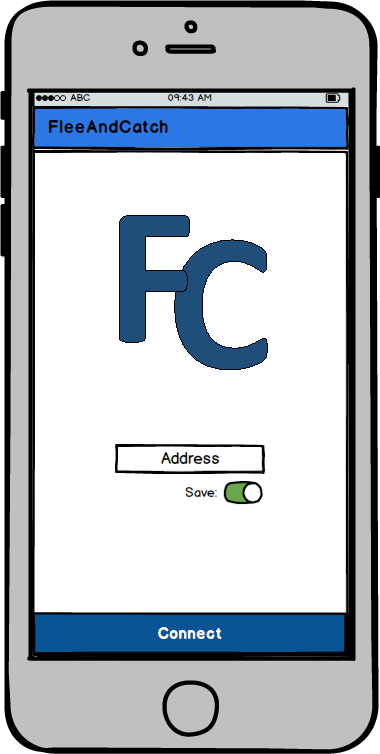
\includegraphics[width=0.25\textwidth]{images/mockups/Connection.png}\label{fig:Connect}}
	\qquad
	\subfloat[Home]{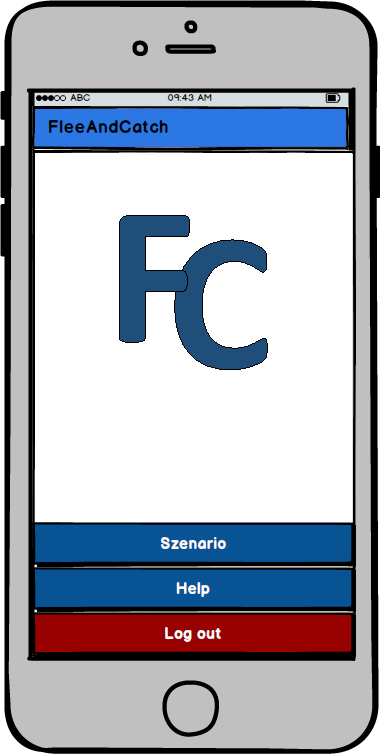
\includegraphics[width=0.25\textwidth]{images/mockups/Home.png}\label{fig:Home}}
	\caption{Mockup Connection}
\end{figure}
\newpage
\begin{verbatim}
\end{verbatim}
\begin{figure}[h]
	\begin{center}
		\includegraphics[width=1\textwidth]{images/use_cases/Connect.png}
	\end{center}
	\caption{Use Case Connection}
	\label{fig:UC_Connect}
\end{figure}

\newpage
\subsubsection{Synchronization}

Der Use Case Synchronization stellt den Datenaustausch der beteiligten Komponenten dar, siehe Abbildung \ref{fig:UC_Synchronization} und \ref{fig:UC_Update}. Hierbei sollen verschiedene Typen unterschieden werden, wobei der komplette Datensatz in Form von allen Szenarien, Robotern, oder eines einzelnen Szenarios, sowie Roboters übertragen werden soll. Dies wird einerseits der Erstellung eines Szenarios dienen, als auch dessen Beobachtung durch den Spectator Modus. Die Übertragung eines einzelnen Roboter dient der Aktualisierung der jeweiligen Daten der Desktopanwendung, sowie der App, um diese laufend aktuell zu halten. Die synchronisierten Daten sollen des Weiteren auf den Komponenten über eine \gls{ui} dargestellt werden können, um die Veränderung der aktuellen Daten zu verdeutlichen, sowie eine verbesserte Steuerung schaffen.\\

\begin{figure}[h]
	\centering
	\subfloat[Log in]{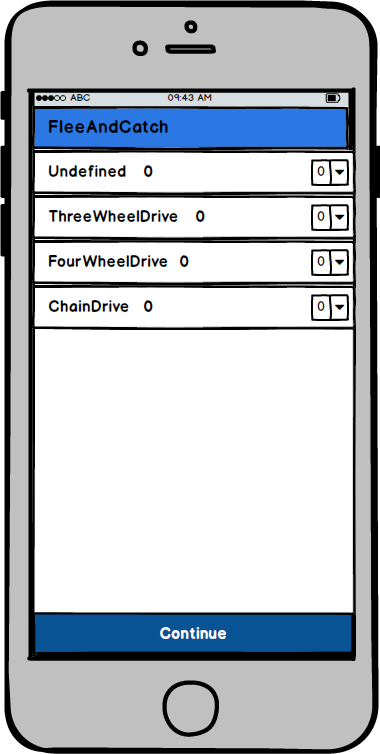
\includegraphics[width=0.25\textwidth]{images/mockups/RobotList.png}\label{fig:Synchronization_1}}
	\qquad
	\subfloat[Home]{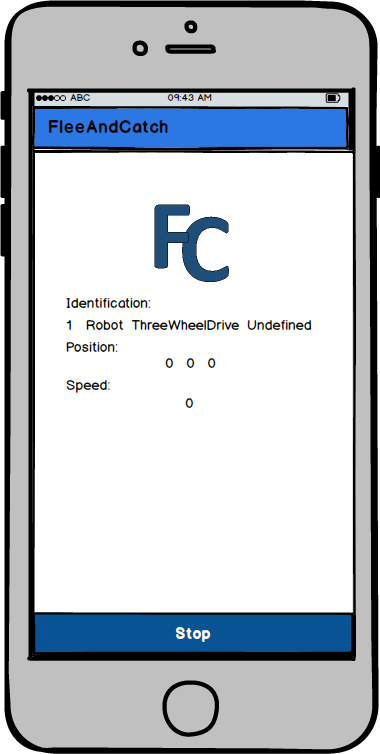
\includegraphics[width=0.25\textwidth]{images/mockups/Control.png}\label{fig:Synchronization_2}}
	\caption{Mockup Synchronization}
\end{figure}
\newpage
\begin{verbatim}
\end{verbatim}
\begin{figure}[h]
	\begin{center}
		\includegraphics[width=0.35\textwidth]{images/use_cases/Synchronization.png}
	\end{center}
	\caption{Use Case Synchronization}
	\label{fig:UC_Synchronization}
\end{figure}
\begin{figure}[h]
	\begin{center}
		\includegraphics[width=0.3\textwidth]{images/use_cases/Update.png}
	\end{center}
	\caption{Use Case Update}
	\label{fig:UC_Update}
\end{figure}

\newpage
\subsubsection{Szenario}

Der Use Case Szenario stellt den Ablauf der definierten Szenarien, zur Steuerung der Roboter dar, siehe Abbildung \ref{fig:UC_Szenario_1}. Der Nutzer soll dabei zu Beginn das gewünschte Szenario, sowie die teilnehmenden Roboter festlegen. Anschließend wird das Szenario durch das Senden eines Kommandos gestartet, welches von der Desktopanwendung initialisiert wird. Dieses Kommando soll laufend wiederholt werden, um aktuelle Daten, wie Steuerungsinformationen an die Roboter weiterzuleiten. Zur Steuerung sollen hierbei eine direkte von einer positionsorientierten unterschieden werden, wobei die Roboter je nach Kommando die direkten Steuerungsinformationen oder eine anzufahrende Position erhalten.\\
Diese Implementierung soll den Vorteil einer Auslagerung der Programmlogik schaffen, indem die Ressourcen der Roboter geschont werden und die Logik zentral in der Desktopanwendung ausgeführt werden kann.\\
 
\begin{figure}[h]
	\centering
	\subfloat[Szenario]{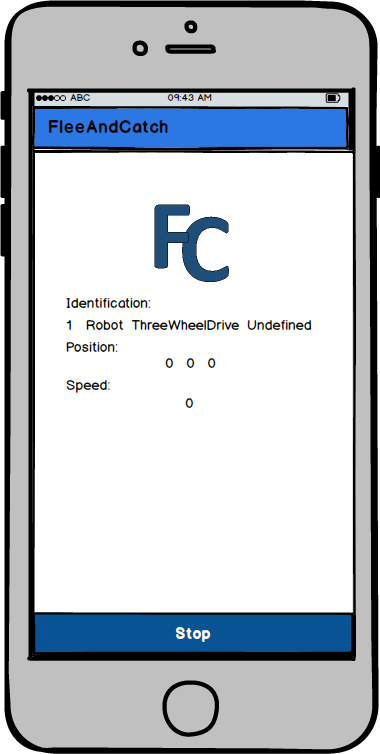
\includegraphics[width=0.25\textwidth]{images/mockups/Control.png}\label{fig:Szenario_1}}
	\qquad
	\subfloat[Spectator]{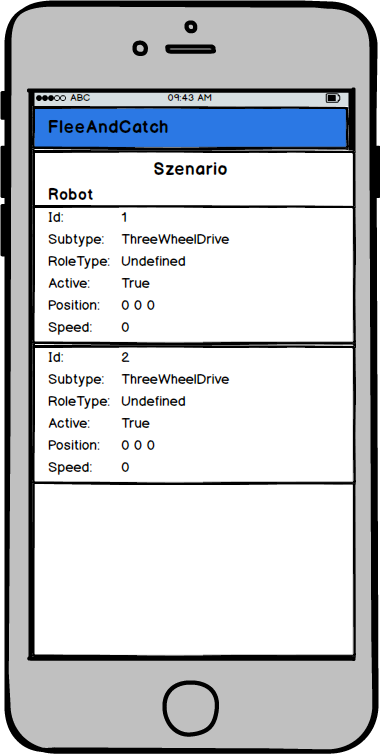
\includegraphics[width=0.25\textwidth]{images/mockups/Spectator.png}\label{fig:Szenario_2}}
	\caption{Mockup Szenario}
\end{figure}
\newpage
\begin{verbatim}
\end{verbatim}
\begin{figure}[h]
	\begin{center}
		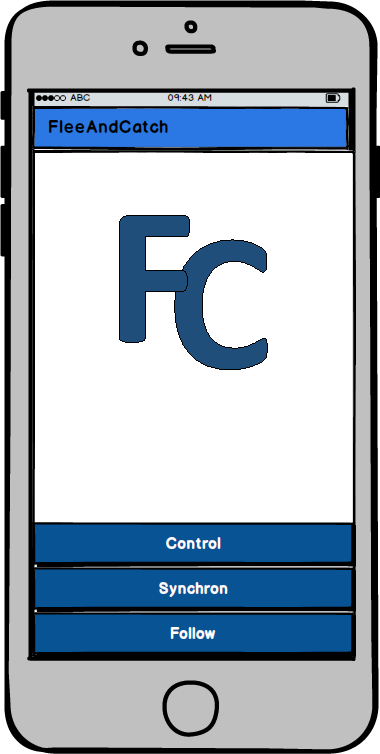
\includegraphics[width=0.425\textwidth]{images/use_cases/Szenario.png}
	\end{center}
	\caption{Use Case Szenario}
	\label{fig:UC_Szenario_1}
\end{figure}
\begin{figure}[h]
	\begin{center}
		\includegraphics[width=0.375\textwidth]{images/use_cases/Spectator.png}
	\end{center}
	\caption{Use Case Spectator}
	\label{fig:UC_Szenario_2}
\end{figure}

\newpage

\subsubsection{Exception}

Der Use Case Exception stellt den Ablauf einer auftretenden Exception in einem Roboter zum Kontext eines Verbindungsverlustes dar, siehe Abbildung \ref{fig:Exception}. Dabei soll die auftretenden Nachricht, sowie die beteiligte Komponente der Desktopanwendung zugesendet werden. Dies soll ein kontrolliertes Schließen eines Szenarios ermöglichen, welches von einer solchen Exception betroffen ist. Die dabei teilnehmenden Komponenten, wie Nutzer und andere Roboter sollen entsprechend zurückgesetzt werden, damit diese für ein neues Szenario zur Verfügung stehen.\\

\begin{figure}[h]
	\begin{center}
		\includegraphics[width=0.5\textwidth]{images/use_cases/Exception.png}
	\end{center}
	\caption{Use Case Exception}
	\label{fig:Exception}
\end{figure}

\newpage
\subsection{Kommunikation}\label{kommunikation}

Die Kommunikation des Schwarmverhalten basiert auf dem Standard für Netzwerkkommunikation, indem über eine \gls{tcp} Schnittstelle Zeichenketten binär versendet werden. Dabei sollen die zu übertragenen Daten als Zeichenkette serialisiert und binär versendet werden, wobei die Gegenstelle die Daten über eine vorliegende Kommandostruktur deserialisiert. Um auf die Daten entsprechend zu reagieren werden diese nach Abhängigkeiten interpretiert. Dies soll über einen Typen realisiert werden, der der jeweiligen Struktur des Kommandos entspricht. Damit die Kommandostruktur als solche von den Komponenten von anderen unterschieden werden kann, sollen diese eine zusätzliche Grundstruktur zur Identifizierung der Schnittstelle, als auch den Kommandos erhalten. 

\paragraph{Connection} stellt das Kommando zur allgemeinen Verbindung dar, wobei eine Verbindung sowohl aufgebaut, als auch abgebaut werden kann. Dazu werden Parameter zur Identifizierung von Komponenten genutzt, die entsprechend auch in weiteren Kommandos ihre Anwendung finden. Die Tabelle \ref{tab:Connection} stellt den allgemeinen Aufbau eines solchen Kommandos dar.

\begin{table}[h]
	\centering
	\begin{tabular}{|p{4cm}|p{8cm}|}
		\hline
		\textbf{Connection} & Definition\\
		\hline
		String id & Stellt den Identifikationsstring dar \\
		String type & Stellte den Typen dar \\
		String apiid & Stellt die verwendete \gls{api} dar \\
		ClientIdentification identification & Stellt das Identifikationsobjekt der Komponente dar \\
		\hline
	\end{tabular}
	\caption[\gls{json} Kommando Connection]{\gls{json} Kommando Connection}
	\label{tab:Connection}
\end{table}

\paragraph{Synchronization} stellt das Kommando zur Synchronization der erfassten Daten zwischen den verschiedenen Komponenten dar. Dabei werden die Daten als Listen mit entsprechenden Szenarien, wie Robotern übertragen. Je nach vorliegendem Typ des Kommandos, können verschiedene Daten übertragen werden, wobei Current einem einzelnen Objekten und die entsprechende Mehrzahl kompletten Datensätzen entspricht.

\begin{table}[h]
	\centering
	\begin{tabular}{|p{4cm}|p{10cm}|}
		\hline
		\textbf{Synchronization} & Definition\\
		\hline
		String id & Stellt den Identifikationsstring dar \\
		String type & Stellte den Typen dar \\
		String apiid & Stellt die verwendete \gls{api} dar \\
		ClientIdentification identification & Stellt das Identifikationsobjekt der Komponente dar \\
		List scenarios & Stellt die aktuellen Szenarien dar, die übertragen werden\\
		List robots & Stellt die aktuellen Roboter dar, die übertragen werden \\
		\hline
	\end{tabular}
	\caption[\gls{json} Kommando Synchronization]{\gls{json} Kommando Synchronization}
	\label{tab:Synchronization}
\end{table}

\paragraph{Scenario} stellt das aktuell ablaufende Szenario dar, dass als Schwarmverhalten nachgeahmt wird. Darin enthalten sind die teilnehmenden Komponenten, sowie deren aktuell erfassten Daten. Zudem sind Steuerungsinformationen enthalten, die zur Orientierung des Schwarms entsprechend dem Kommando dienen. Diese verändern sich je nach Typen des Szenarios und können in verschiedenen Kontexten kommuniziert werden, um ein unterschiedliches Ergebnis zu erreichen.\\

\begin{table}[h]
	\centering
	\begin{tabular}{|p{4cm}|p{8cm}|}
		\hline
		\textbf{Scenario} & Definition\\
		\hline
		String id & Stellt den Identifikationsstring dar \\
		String type & Stellte den Typen dar \\
		String apiid & Stellt die verwendete \gls{api} dar \\
		ClientIdentification identification & Stellt das Identifikationsobjekt der Komponente dar \\
		Scenario scenarios & Stellt das aktuell ablaufende Szenario dar \\
		\hline
	\end{tabular}
	\caption[\gls{json} Kommando Scenario]{\gls{json} Kommando Scenario}
	\label{tab:Szenario}
\end{table}

\paragraph{Exception} stellt das Kommando zur Abhandlung eines Fehlverhaltens einer Komponente dar, die anderen Komponenten mitgeteilt werden kann. Sie enthält Informationen zur verursachenden Komponente, sowie des auftretenden Fehlers, der behandelt wird. Verwendung findet die Fehlerweiterleitung im Verbindungsverlust des Roboters, damit andere Teilnehmer über das Abmelden des entsprechenden Roboters in Kenntnis gesetzt werden und das Szenario beenden.

\begin{table}[h]
	\centering
	\begin{tabular}{|p{4cm}|p{8cm}|}
		\hline
		\textbf{Exception} & Definition\\
		\hline
		String id & Stellt den Identifikationsstring dar \\
		String type & Stellte den Typen dar \\
		String apiid & Stellt die verwendete \gls{api} dar \\
		ClientIdentification identification & Stellt das Identifikationsobjekt der Komponente dar \\
		Exception exception & Stellt die aktuelle Execption dar, die im Roboter auftritt \\
		\hline
	\end{tabular}
	\caption[\gls{json} Kommando Exception]{\gls{json} Kommando Exception}
	\label{tab:Exception}
\end{table}

\newpage
\paragraph{Control} stellt das Kommando zur direkten Steuerung eines Roboters dar. Hierbei werden Steuerungsinformationen, wie Geschwindigkeit und Ausrichtung übertragen, um den Roboter entsprechend seiner aktuellen Position relativ zu steuern. Dies findet Anwendung in einer direkten Steuerung, als auch im Schwarmverhalten zur Steuerung des Nutzer abhängigen Roboters.

\begin{table}[h]
	\centering
	\begin{tabular}{|p{4cm}|p{8cm}|}
		\hline
		\textbf{Control} & Definition\\
		\hline
		String id & Stellt den Identifikationsstring dar \\
		String type & Stellte den Typen dar \\
		String apiid & Stellt die verwendete \gls{api} dar \\
		ClientIdentification identification & Stellt das Identifikationsobjekt der Komponente dar \\
		Robot robot & Stellt den aktuellen Roboter dar\\
		Steering steering & Stellt die aktuellen Steuerungsinformationen dar \\
		\hline
	\end{tabular}
	\caption[\gls{json} Kommando Control]{\gls{json} Kommando Control}
	\label{tab:Control}
\end{table}

\paragraph{Position} stellt das Kommando zur indirekten Steuerung eines Roboters dar. Hierbei werden Positionsdaten übertragen, die der autonomen Navigation des Roboters dienen. Um eine entsprechende Geschwindigkeit zu erhalten, kann zudem ein Geschwindigkeitswert angefügt werden, der abhängig des Roboters gesetzt wird.

\begin{table}[h]
	\centering
	\begin{tabular}{|p{4cm}|p{8cm}|}
		\hline
		\textbf{Position} & Definition\\
		\hline
		String id & Stellt den Identifikationsstring dar \\
		String type & Stellte den Typen dar \\
		String apiid & Stellt die verwendete \gls{api} dar \\
		ClientIdentification identification & Stellt das Identifikationsobjekt der Komponente dar \\
		Robot robot & Stellt den aktuellen Roboter dar\\
		Position position &  Stellt die anzufahrende Position dar\\
		Speed speed & Stellt die einzustellende Geschwindigkeit dar\\
		\hline
	\end{tabular}
	\caption[\gls{json} Kommando Position]{\gls{json} Kommando Position}
	\label{tab:Position}
\end{table}